% ====================================================================
% Unofficial McGill Masters Thesis Template
% Copyright (C) 2018  Xavier Capaldi (xcapaldi @ Github)
%
% This template is free: you can redistribute it and/or modify
% it under the terms of the GNU General Public License as published by
% the Free Software Foundation, either version 3 of the License, or
% (at your option) any later version.
%
% This template is distributed in the hope that it will be useful,
% but WITHOUT ANY WARRANTY; without even the implied warranty of
% MERCHANTABILITY or FITNESS FOR A PARTICULAR PURPOSE.  See the
% GNU General Public License for more details.
% ====================================================================

% ---
% Masters thesis should be less than 100 (soft cap) or 150 (hard cap)
% That being said, it should be concise and follow all norms of academic writing
% Appendices can be used to present supplementary or raw data
% Script and Page Format: conventional font, size 12-point, 12 characters per inch, 1.5 or 2 line spacing, left and right margins 1 inch
% footnotes, references and appendices should follow standard style of your discipline
% avoid full-page images and plots
% ---

\documentclass[12pt,oneside,openany,letterpaper]{book} % book defaults: twoside, titlepage, openright (always start chapters on odd pages) These are good for printing. Otherwise use settings here. Draft makes it so that images are not rendered (just a box)
\usepackage{mystyle} % call my custom style file containing all the used packages and settings
%\includeonly{./tex/section-a} % use to compile only sections of document

\begin{document}

\frontmatter % the following pages will be roman numerals
% ----------
% Title Page
% ----------
% ====================================================================
% Unofficial McGill Masters Thesis Template
% Copyright (C) 2018  Xavier Capaldi (xcapaldi @ Github)
%
% This template is free: you can redistribute it and/or modify
% it under the terms of the GNU General Public License as published by
% the Free Software Foundation, either version 3 of the License, or
% (at your option) any later version.
%
% This template is distributed in the hope that it will be useful,
% but WITHOUT ANY WARRANTY; without even the implied warranty of
% MERCHANTABILITY or FITNESS FOR A PARTICULAR PURPOSE.  See the
% GNU General Public License for more details.
% ====================================================================

\begin{titlepage}
    \begin{center}
        \vspace*{1cm}

        \huge
        \textbf{TITLE OF THESIS}

        \vspace{0.5cm}
        \large
%        SUBTITLE IF NECESSARY

        \vspace{1.5cm}

        \textbf{YOUR NAME}

        \vfill

        A thesis submitted to McGill University in partial fulfillment of the requirements of the degree of \textbf{Master of Science}

        \vspace{0.8cm}
       
%       I cannot provide the McGill logo with this template but you can get a copy as a McGill graduate student (i.e. staff).
%       Get the logo from here: https://www.mcgill.ca/visual-identity/download-mcgill-logo
       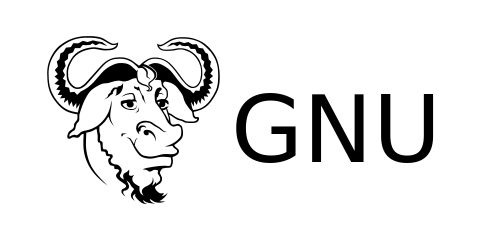
\includegraphics[scale=0.5]{logo.png}

        \large
        Department of YOUR DEPARTMENT\\
        McGill University\\
        Canada, Qu\'{e}bec\\
        DATE

        \vspace{1.5cm}

        \textcopyright{} YEAR YOUR NAME\\
        All Rights Reserved
    \end{center}
\end{titlepage}
 % or use defaults %%
% title of thesis
% student's name and unit (department)
% month and year of submission
% "A thesis submitted to McGill University in partial fulfillment of the requirements of the degree of ..."
% the universal copyright notice "\textcopyright" (this will require the textcomp package if you want it to look nice) followed by the student's name and the year the thesis was submitted
% -----------------
% Table of Contents
% -----------------
% must be detailed
\setcounter{tocdepth}{3} % change this to control the depth of the generated table of contents
\tableofcontents %%
%\listoffigures % not sure these are necessary
%\listoftables % not sure these are necessary
% --------
% Abstract
% ---------
% ====================================================================
% Unofficial McGill Masters Thesis Template
% Copyright (C) 2018  Xavier Capaldi (xcapaldi @ Github)
%
% This template is free: you can redistribute it and/or modify
% it under the terms of the GNU General Public License as published by
% the Free Software Foundation, either version 3 of the License, or
% (at your option) any later version.
%
% This template is distributed in the hope that it will be useful,
% but WITHOUT ANY WARRANTY; without even the implied warranty of
% MERCHANTABILITY or FITNESS FOR A PARTICULAR PURPOSE.  See the
% GNU General Public License for more details.
% ====================================================================

\chapter{Abstract}

\lipsum

% ====================================================================
% Unofficial McGill Masters Thesis Template
% Copyright (C) 2018  Xavier Capaldi (xcapaldi @ Github)
%
% This template is free: you can redistribute it and/or modify
% it under the terms of the GNU General Public License as published by
% the Free Software Foundation, either version 3 of the License, or
% (at your option) any later version.
%
% This template is distributed in the hope that it will be useful,
% but WITHOUT ANY WARRANTY; without even the implied warranty of
% MERCHANTABILITY or FITNESS FOR A PARTICULAR PURPOSE.  See the
% GNU General Public License for more details.
% ====================================================================

\chapter{Abrégé}

If you use XeLaTeX and the packages I recommend, you can simply type your accents I have done in the title here.

\lipsum

% brief abstract in both English and French
% ----------------
% Acknowledgements
% ----------------
% ====================================================================
% Unofficial McGill Masters Thesis Template
% Copyright (C) 2018  Xavier Capaldi (xcapaldi @ Github)
%
% This template is free: you can redistribute it and/or modify
% it under the terms of the GNU General Public License as published by
% the Free Software Foundation, either version 3 of the License, or
% (at your option) any later version.
%
% This template is distributed in the hope that it will be useful,
% but WITHOUT ANY WARRANTY; without even the implied warranty of
% MERCHANTABILITY or FITNESS FOR A PARTICULAR PURPOSE.  See the
% GNU General Public License for more details.
% ====================================================================

\chapter{Acknowledgements}
% recognize the supervision and advice given by the thesis supervisor(s) and advisors
% also, you must declare the extent to which assistance (paid and unpaid) has been given by members of staff, fellow students, research assistants, technicians, or others in collection of materials and data, the design and construction of apparatus, the performance of experiments, analysis of data, and the preparation of the thesis (including editorial help)

\lipsum

 %%
% recognize the supervision and advice given by the thesis supervisor(s) and advisors
% also, you must declare the extent to which assistance (paid and unpaid) has been given by members of staff, fellow students, research assistants, technicians, or others in collection of materials and data, the design and construction of apparatus, the performance of experiments, analysis of data, and the preparation of the thesis (including editorial help)
% -----------------------------------------
% Statement of Originality and Contribution
% -----------------------------------------
% ====================================================================
% Unofficial McGill Masters Thesis Template
% Copyright (C) 2018  Xavier Capaldi (xcapaldi @ Github)
%
% This template is free: you can redistribute it and/or modify
% it under the terms of the GNU General Public License as published by
% the Free Software Foundation, either version 3 of the License, or
% (at your option) any later version.
%
% This template is distributed in the hope that it will be useful,
% but WITHOUT ANY WARRANTY; without even the implied warranty of
% MERCHANTABILITY or FITNESS FOR A PARTICULAR PURPOSE.  See the
% GNU General Public License for more details.
% ====================================================================

\chapter{Statement of Originality and Contribution}
% clearly state the elements of the thesis that are considered original scholarship and distinct contributions to knowledge
% contributions of the student to each chapter must be explicitly stated
% contributions of any co-authors to each chapter must be explicitly stated 

\lipsum
 
% clearly state the elements of the thesis that are considered original scholarship and distinct contributions to knowledge
% contributions of the student to each chapter must be explicitly stated
% contributions of any co-authors to each chapter must be explicitly stated

\mainmatter % book specific that specifies to switch page numbering
% ------------
% Introduction
% ------------
% clearly state the rational and objectives of the research
\chapter{Introduction}
  % ====================================================================
% Unofficial McGill Masters Thesis Template
% Copyright (C) 2018  Xavier Capaldi (xcapaldi @ Github)
%
% This template is free: you can redistribute it and/or modify
% it under the terms of the GNU General Public License as published by
% the Free Software Foundation, either version 3 of the License, or
% (at your option) any later version.
%
% This template is distributed in the hope that it will be useful,
% but WITHOUT ANY WARRANTY; without even the implied warranty of
% MERCHANTABILITY or FITNESS FOR A PARTICULAR PURPOSE.  See the
% GNU General Public License for more details.
% ====================================================================

% clearly state the rational and objectives of the research

\lipsum

% -----------------
% Literature Review
% -----------------
% literature review must be comprehensive and in line with disciplinary expectations
\chapter{Review of XYZ}
  % ====================================================================
% Unofficial McGill Masters Thesis Template
% Copyright (C) 2018  Xavier Capaldi (xcapaldi @ Github)
%
% This template is free: you can redistribute it and/or modify
% it under the terms of the GNU General Public License as published by
% the Free Software Foundation, either version 3 of the License, or
% (at your option) any later version.
%
% This template is distributed in the hope that it will be useful,
% but WITHOUT ANY WARRANTY; without even the implied warranty of
% MERCHANTABILITY or FITNESS FOR A PARTICULAR PURPOSE.  See the
% GNU General Public License for more details.
% ====================================================================

\section{Review X}
\label{review-x}

\lipsum

\cite{zhu2013}

  % ====================================================================
% Unofficial McGill Masters Thesis Template
% Copyright (C) 2018  Xavier Capaldi (xcapaldi @ Github)
%
% This template is free: you can redistribute it and/or modify
% it under the terms of the GNU General Public License as published by
% the Free Software Foundation, either version 3 of the License, or
% (at your option) any later version.
%
% This template is distributed in the hope that it will be useful,
% but WITHOUT ANY WARRANTY; without even the implied warranty of
% MERCHANTABILITY or FITNESS FOR A PARTICULAR PURPOSE.  See the
% GNU General Public License for more details.
% ====================================================================

\section{Review Y}
\label{review-y}

\lipsum

\cite{mao2005}

  % ====================================================================
% Unofficial McGill Masters Thesis Template
% Copyright (C) 2018  Xavier Capaldi (xcapaldi @ Github)
%
% This template is free: you can redistribute it and/or modify
% it under the terms of the GNU General Public License as published by
% the Free Software Foundation, either version 3 of the License, or
% (at your option) any later version.
%
% This template is distributed in the hope that it will be useful,
% but WITHOUT ANY WARRANTY; without even the implied warranty of
% MERCHANTABILITY or FITNESS FOR A PARTICULAR PURPOSE.  See the
% GNU General Public License for more details.
% ====================================================================

\section{Review Z}
\label{review-z}

\lipsum

\cite{sedlazeck2018}


% --------------
% Body of Thesis
% --------------
% should contain sections on methodology and research finding
% -----------
% Methodology
% -----------
\chapter{Methodology}
  % ====================================================================
% Unofficial McGill Masters Thesis Template
% Copyright (C) 2018  Xavier Capaldi (xcapaldi @ Github)
%
% This template is free: you can redistribute it and/or modify
% it under the terms of the GNU General Public License as published by
% the Free Software Foundation, either version 3 of the License, or
% (at your option) any later version.
%
% This template is distributed in the hope that it will be useful,
% but WITHOUT ANY WARRANTY; without even the implied warranty of
% MERCHANTABILITY or FITNESS FOR A PARTICULAR PURPOSE.  See the
% GNU General Public License for more details.
% ====================================================================

\section{Methodology X}
\label{method-x}

\lipsum

  % ====================================================================
% Unofficial McGill Masters Thesis Template
% Copyright (C) 2018  Xavier Capaldi (xcapaldi @ Github)
%
% This template is free: you can redistribute it and/or modify
% it under the terms of the GNU General Public License as published by
% the Free Software Foundation, either version 3 of the License, or
% (at your option) any later version.
%
% This template is distributed in the hope that it will be useful,
% but WITHOUT ANY WARRANTY; without even the implied warranty of
% MERCHANTABILITY or FITNESS FOR A PARTICULAR PURPOSE.  See the
% GNU General Public License for more details.
% ====================================================================

\section{Methodology Y}
\label{method-y}

\lipsum

  % ====================================================================
% Unofficial McGill Masters Thesis Template
% Copyright (C) 2018  Xavier Capaldi (xcapaldi @ Github)
%
% This template is free: you can redistribute it and/or modify
% it under the terms of the GNU General Public License as published by
% the Free Software Foundation, either version 3 of the License, or
% (at your option) any later version.
%
% This template is distributed in the hope that it will be useful,
% but WITHOUT ANY WARRANTY; without even the implied warranty of
% MERCHANTABILITY or FITNESS FOR A PARTICULAR PURPOSE.  See the
% GNU General Public License for more details.
% ====================================================================

\section{Methodology Z}
\label{method-z}

\lipsum

% --------------------------------
% Scholarly Discussion of Findings
% --------------------------------
\chapter{Results}
  % ====================================================================
% Unofficial McGill Masters Thesis Template
% Copyright (C) 2018  Xavier Capaldi (xcapaldi @ Github)
%
% This template is free: you can redistribute it and/or modify
% it under the terms of the GNU General Public License as published by
% the Free Software Foundation, either version 3 of the License, or
% (at your option) any later version.
%
% This template is distributed in the hope that it will be useful,
% but WITHOUT ANY WARRANTY; without even the implied warranty of
% MERCHANTABILITY or FITNESS FOR A PARTICULAR PURPOSE.  See the
% GNU General Public License for more details.
% ====================================================================

\lipsum


% ----------------------------
% Final Conclusion and Summary
% ----------------------------
% State how the objectives of the research were met and discuss implications of findings
\chapter{Conclusion}
  % ====================================================================
% Unofficial McGill Masters Thesis Template
% Copyright (C) 2018  Xavier Capaldi (xcapaldi @ Github)
%
% This template is free: you can redistribute it and/or modify
% it under the terms of the GNU General Public License as published by
% the Free Software Foundation, either version 3 of the License, or
% (at your option) any later version.
%
% This template is distributed in the hope that it will be useful,
% but WITHOUT ANY WARRANTY; without even the implied warranty of
% MERCHANTABILITY or FITNESS FOR A PARTICULAR PURPOSE.  See the
% GNU General Public License for more details.
% ====================================================================

% State how the objectives of the research were met and discuss implications of findings 

\lipsum

%\clearpage
%\appendix
  %\include{./tex/myappendix}

% ---------------------------------------
% Thorough Bibliography or Reference List
% ---------------------------------------
\printbibliography[title={References},heading=bibintoc]
\end{document}
